\begin{pa} \label{PA:10.8} 
  Suppose we would like to find the maxima and minima of the function
  $f(x,y) = 2x + y$ on the circle $x^2+y^2=5$, as shown on the left of
  Figure \ref{F:10.8.preview}.  Also shown on the right of Figure
  \ref{F:10.8.preview} are some contour lines of $f(x,y)$.

  \begin{figure}[ht]
  \begin{center}
    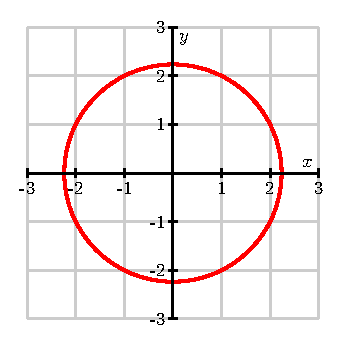
\includegraphics{figures/fig_10_8_preview.eps}
    \hspace*{20pt}
    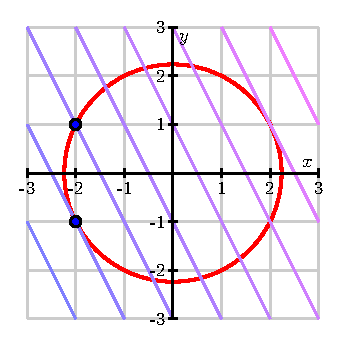
\includegraphics{figures/fig_10_8_preview_contour.eps}
  \end{center}
  \caption{The circle $x^2+y^2=5$ and contours of $f(x,y) = 2x+y$.}
  \label{F:10.8.preview}
\end{figure}

  \ba
\item Find the gradient $\nabla f$.
\item On the right of Figure \ref{F:10.8.preview}, sketch the gradient
  $\nabla f(-2,1)$.  Also, sketch a vector $\vv$ tangent to the circle
  $x^2+y^2 = 5$.  
\item For the vector $\vv$ you have drawn, what is the sign of $\nabla
  f(-2,1)\cdot\vv$.  
\item Remember that we want to find the extrema of $f(x,y)$
  as we move around the circle.  As we move on the circle from the
  point $(-2,1)$ in the direction of $\vv$, what happens to the value
  of $f$?  Can $(-2,1)$ be an extremum for $f$?
\item Now sketch the gradient $\nabla f(-2,-1)$ along with a vector
  $\vv$ tangent to the circle at $(-2,-1)$.  What is the value of
  $\nabla f(-2,-1)\cdot\vv$?  What does this say about the value of
  $f$ as we move on the circle from the point $(-2,-1)$ in the
  direction of $\vv$?
\item Continuing this geometric way of thinking, determine
  the extrema of $f$ on the circle $x^2+y^2=5$.
\item The circle is defined by the equation $x^2+y^2 =5$.  As such, it
  is itself a contour of the function $g(x,y) = x^2 + y^2$.  On Figure
  \ref{F:10.8.preview.draw}, sketch the vectors $\nabla f$ and $\nabla
  g$ at the points $(-2,1)$, $(-1,-2)$, $(1,-2)$, and $(2,1)$.  What
  special condition occurs at the extrema?

\begin{figure}[ht]
  \begin{center}
    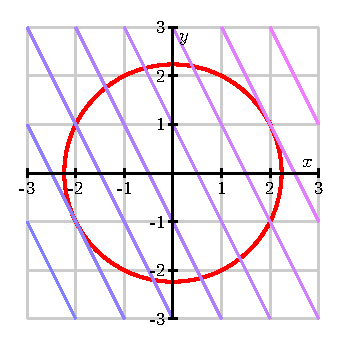
\includegraphics{figures/fig_10_8_preview_draw.eps}
  \end{center}
  \caption{The gradient of $f$ and $g$}
  \label{F:10.8.preview.draw}
\end{figure}
  \ea
\end{pa} 
\afterpa 